
\begin{figure}[!htbp]
\begin{center}
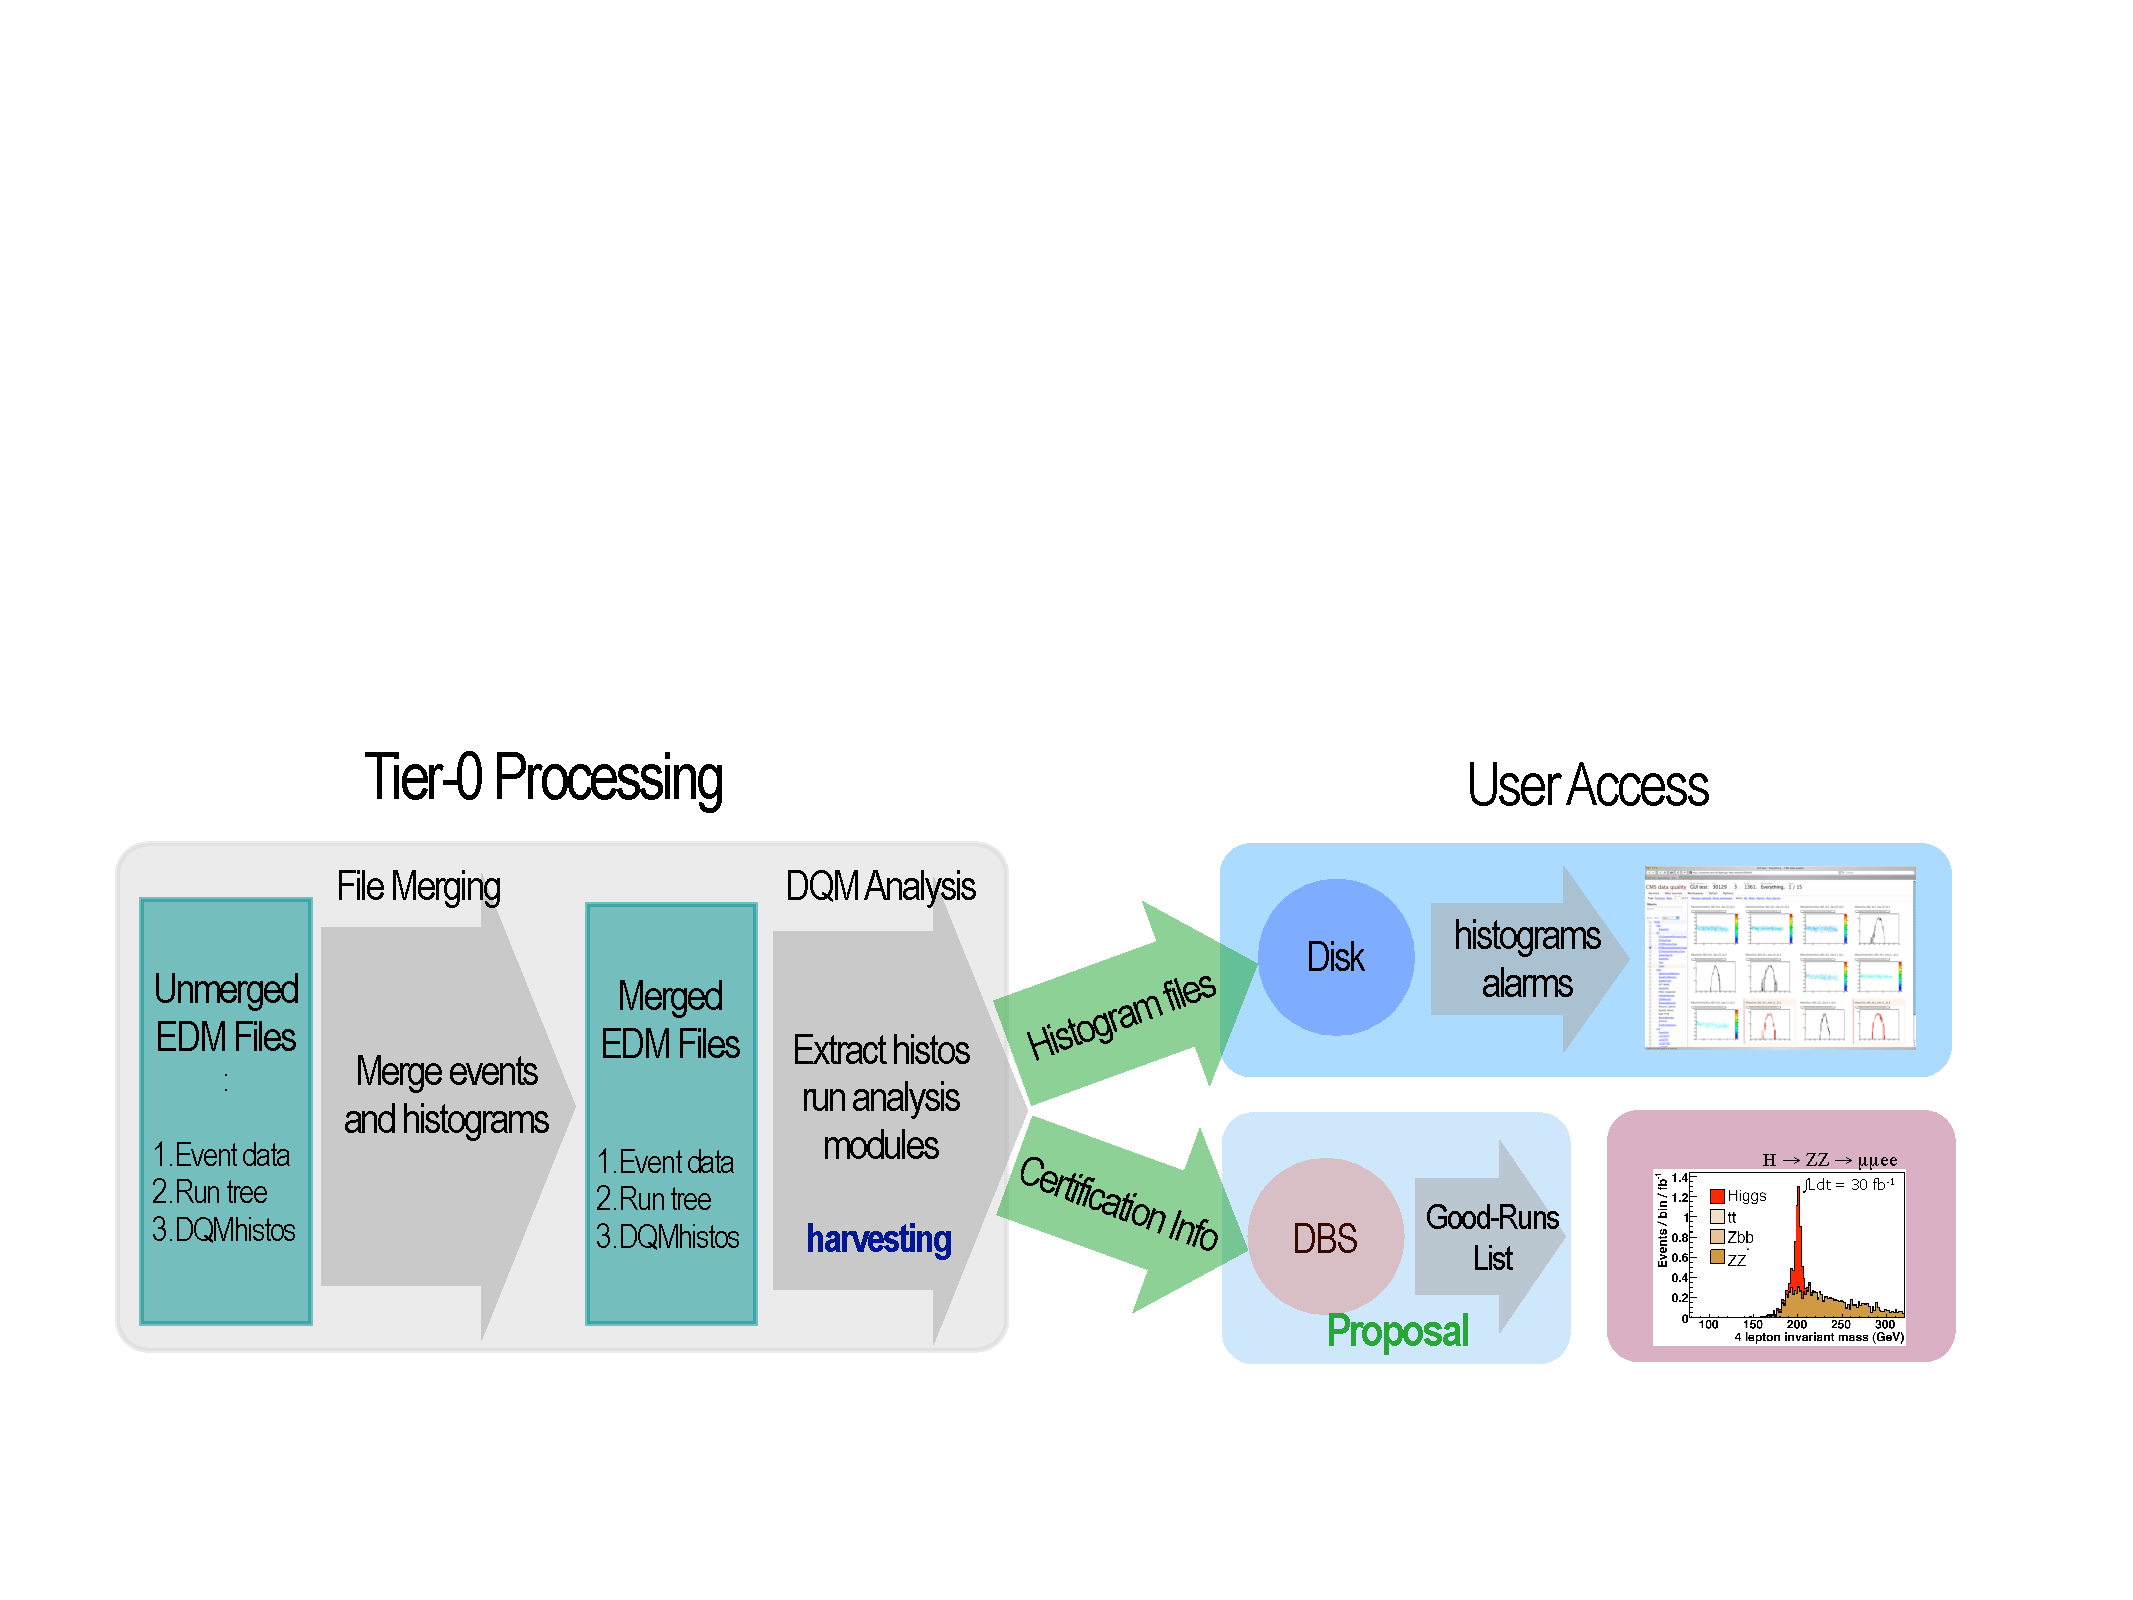
\includegraphics[width=0.9\textwidth]{dqm_tier0}
\caption{DQM data flow at Tier-0}
\end{center}
\label{fig:dqmoffline}
\end{figure}


\subsection{Prompt Reconstruction Monitoring}


Tier-0 DQM processing consists of two steps. In the first step
the histograms are created, filled with event information and stored 
in the EDM job output files (along with the processed events).
In a second step, the histograms are extracted from the EDM files.
They are merged (summed) together, and analysis and
quality test steps are performed. The second step includes
the calculation of physics data certification decisions.

At the end of the second step the output histograms are stored in files 
which are transfered to the file archive on the histogram DQM GUI server machine
and the certification information is written to the conditions database and into DBS.

\subsubsection{Histogram creation and filling}

% here put some details about:
DQM histograms creation, filling, storage in EDM files 
and subsequent summation of histograms during EDM file merge.
            + Tier-0, DQMOffline (package and sequence definitions), DPG, POG

\subsubsection{Harvesting step}

\begin{itemize}
\item{Extraction and Quality testing}

\item{Physics Data Certification} 

refer to section \ref{sec:certification})


\end{itemize}

\subsection{Release Validation}

\subsection{Calibration Monitoring}

\begin{figure}[!htbp]
\begin{center}
%\includegraphics[width=0.9\textwidth]{dqm_alca}
\caption{Envisaged DQM data flow for calibration and alignment purposes.}
\end{center}
\label{fig:dqmalca}
\end{figure}

Calibration workflow layout and integration (mostly CAF)

\subsection{DQM at the CAF}
\label{sec:caf}

Define support of CAF activity by DQM group.
Handshake between root-file output and offline DQM GUI

%==========================================================
% this subsection is common to all sections, please fill in 
\subsection{Offline DQM Integration and Operation}

\subsubsection*{Integration}

\subsubsection*{Operation}
